\section{Experiments}\label{sec:experiments}

Using the model zoo of \citet{wang2025hybrid} (\S\ref{ssec:model_zoo}), we evaluate all 30 configurations on 10 benchmarks plus supplementary COPA ($n = 100$) at 1.3B scale unless noted. Results at 340M appear in scale analyses. Recall: h$k$-1 denotes one attention layer per $k{+}1$ layers; h3-1 = 25\% attention.

\subsection{Per-Example Divergence}\label{ssec:per_example}

Do architectures converge by improving on the same examples? We compare each architecture's pure-recurrent baseline against its h3-1 hybrid on 5{,}153 LAMBADA examples, classifying each as helped, hurt, or unchanged. Although the decomposition is binary, it captures genuine separation in the continuous confidence space (Cohen's $d = 0.73$--$0.92$ between helped and hurt on LAMBADA; cross-benchmark details in Appendix~\ref{app:cm_cross}). Binarization discards confidence magnitude, so we supplement with continuous confidence margin analysis (Appendix~\ref{app:confidence_margin}) and verify that low Jaccard persists under continuous thresholds (Appendix~\ref{app:continuous_jaccard}).

\begin{figure}[t]
\centering
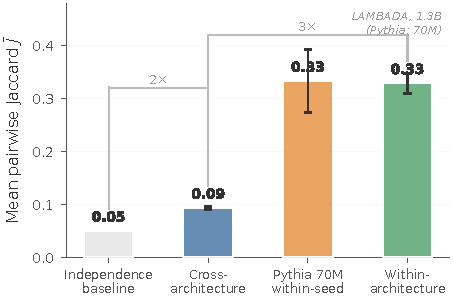
\includegraphics[width=\columnwidth]{figures/fig_jaccard_hierarchy.pdf}
\caption{Jaccard hierarchy on LAMBADA (1.3B). Cross-architecture overlap ($\bar{J} \approx 0.09$) is $2\times$ the independence baseline but only one-third of within-architecture overlap ($\bar{J} \approx 0.33$). Pythia 70M within-seed Jaccard (different scale) falls at a comparable level. Error bars show the helped--hurt range.}
\label{fig:jaccard_hierarchy}
\end{figure}

\begin{figure*}[t]
\centering
\includegraphics[width=0.75\textwidth]{figures/fig3_alpha_routing.pdf}
\caption{(a) Per-example ambiguity $\alpha$ varies $2\times$ across task types. (b) Confidence-based routing gains track $\alpha$: effective when multiplicity is high (LAMBADA) but counterproductive when low (PIQA). 1.3B, h3-1.}
\label{fig:alpha_routing}
\end{figure*}

Each architecture displays a distinct profile of per-example changes (Figure~\ref{fig:per_example_bars}). GDN loses a net 153 examples (462 helped, 615 hurt), RetNet loses 69 (426/495), and HGRN2 gains 153 (548/395; full counts in Appendix~\ref{app:per_example_counts}). HGRN2 is the only architecture for which adding attention yields a net per-example benefit. Pairwise Jaccard similarity is low: mean $\bar{J} \leq 0.10$, indicating ${\sim}90$\% non-overlap. Overlap significantly exceeds the independence baseline ($J_{\text{null}} \approx 0.05$, all $z > 5.9$, $p < .0001$; Appendix~\ref{app:jaccard_permutation}), plausibly reflecting shared sensitivity to example difficulty. Normalizing by $J_{\max}$, observed overlap reaches only 6--7\% of the achievable range above chance (Appendix~\ref{app:normalized_es}), confirming that low Jaccard cannot be attributed to set-size constraints.


\paragraph{Confidence margin predictor.} Pure-model confidence on the target token predicts which examples will be affected (AUC 0.70--0.74, a non-parametric measure equivalent to Mann-Whitney $U$; Appendix~\ref{app:confidence_margin}): rescue thresholds (the confidence below which wrong answers are likely corrected by attention) are architecture-invariant (1\% spread) but disruption thresholds (the confidence above which correct answers become vulnerable) vary 47\%, explaining cross-architecture Jaccard divergence (Appendix~\ref{app:prediction_framework}). Calibration differences account for less than half the threshold spread (Appendix~\ref{app:calibration}). The rescue pattern generalizes across three benchmarks ($d = 0.13$--$0.60$; Appendix~\ref{app:cm_cross}); disruption is weaker on reasoning tasks (Appendix~\ref{app:boolq}). This structured disagreement constitutes predictive multiplicity \citep{marx2020predictive} under architectural variation.

\paragraph{Confidence-based routing.} As an illustrative case study, the rescue-threshold asymmetry suggests a routing strategy: select the architecture whose pure-model confidence best predicts successful rescue. On LAMBADA, this outperforms majority vote by $+5.3$\,pp (SD $= 0.4$\,pp, 10 cross-validated splits), extracting 36\% of the oracle gap (oracle = 65.5\%; Appendix~\ref{app:complementarity}). On ARC-Easy, gains are modest ($+1.0$\,pp, SD $= 0.5$\,pp); on HellaSwag, routing provides no benefit ($-0.02$\,pp, $p = .89$); on PIQA, it is significantly negative ($-0.6$\,pp, $p = .006$). Routing works when multiplicity is high ($\alpha = 0.30$, LAMBADA) and a clear rescue-threshold signal exists, but is counterproductive when multiplicity is low ($\alpha = 0.14$, PIQA). A natural comparison (average-logits ensemble) is left to future work as it requires simultaneous inference across all architectures.

\paragraph{Complementarity structure.} Table~\ref{tab:complementarity} decomposes the three-architecture vote on each example. On LAMBADA, 15.1\% of examples are majority-exploitable (2/3 correct) and 14.5\% are majority-hostile (1/3 correct)---a near-even split yielding a majority-vote exploitation ratio of only ${\sim}51$\%. The oracle exploits both categories, explaining the large oracle--MV gap ($+14$\,pp on LAMBADA). This structural constraint is stable across attention ratios (51--54\% on LAMBADA across all five configurations; Appendix~\ref{app:complementarity}).

\begin{table}[t]
\centering
\small
\caption{Complementarity decomposition at 1.3B h3-1. Fractions of examples where $k$ of 3 architectures answer correctly. MV expl.: fraction of non-unanimous examples where majority vote is correct.}
\label{tab:complementarity}
\begin{tabular}{@{}lccccr@{}}
\toprule
Benchmark & 3/3 & 2/3 & 1/3 & 0/3 & MV expl. \\
\midrule
LAMBADA & .361 & .151 & .145 & .343 & 51.1\% \\
HellaSwag & .519 & .078 & .073 & .331 & 51.6\% \\
ARC-Easy & .603 & .107 & .103 & .187 & 50.9\% \\
\bottomrule
\end{tabular}
\end{table}

\paragraph{Multiplicity variation.} Extending to HellaSwag ($N = 10{,}042$) and PIQA ($N = 1{,}838$) reveals that multiplicity varies systematically across tasks (Table~\ref{tab:multiplicity}). Ambiguity $\alpha$ \citep{marx2020predictive} ranges from 0.14 (PIQA) through 0.15 (HellaSwag) and 0.21 (ARC-Easy; Appendix~\ref{app:arceasy}) to 0.30 (LAMBADA). Format does not drive this ordering: HellaSwag (four-way) and PIQA (two-choice) produce nearly identical $\alpha$ despite different answer-space sizes ($\rho = -0.60$, $p = .24$ with task accuracy). This suggests multiplicity is associated with cognitive demands rather than evaluation format, though the confound cannot be fully resolved (Limitations). Bootstrap 95\% CIs confirm the ordering (all non-overlapping except PIQA--HellaSwag; Table~\ref{tab:arceasy_ambiguity}). Pairwise Jaccard remains uniformly low ($\bar{J} \leq 0.10$, all $p < .01$), indicating architectures affect different examples regardless of how many are affected. Within each benchmark, $\alpha$ is stable across attention ratios (variation $< 0.03$) but differs $2\times$ across task types, confirming that multiplicity magnitude depends on task, not attention ratio \citep[cf.][]{gorbett2026crossmodel}.

\begin{figure}[t]
\centering
\includegraphics[width=\columnwidth]{figures/fig2_task_specificity.pdf}
\caption{Spearman $\rho$ between attention ratio and cross-architecture $\sigma$ for each benchmark at 1.3B scale. LAMBADA ($\rho = -1.0$; BCa 95\% CI $[-1.0,\,-0.7]$, heuristic) is the only benchmark whose CI excludes zero. Bootstrap CI is heuristic given $n = 3$ architectures.}
\label{fig:task_specificity}
\end{figure}

\begin{figure*}[t]
\centering
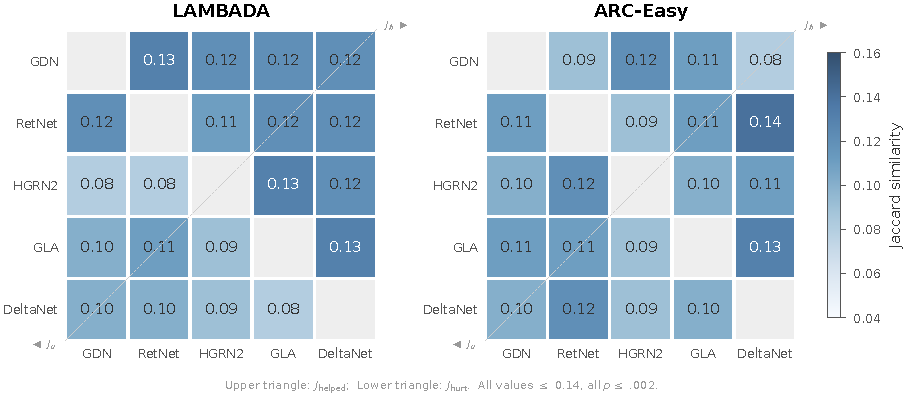
\includegraphics[width=0.75\textwidth]{figures/jaccard_heatmap_5arch.pdf}
\caption{Pairwise Jaccard heatmap across five architectures (340M, h3-1), where helped (hurt) examples are those correct only with (without) attention. Upper triangle: $J_{\text{helped}}$; lower triangle: $J_{\text{hurt}}$. All values $\leq 0.14$, all permutation tests $p < .005$. HellaSwag and PIQA results in Appendix~\ref{app:extended_arch}.}
\label{fig:jaccard_heatmap_5arch}
\end{figure*}

\begin{table}[t]
\centering
\small
\caption{Predictive multiplicity at 1.3B, h3-1. $\alpha$: ambiguity \citep{marx2020predictive}; $\bar{J}$: mean pairwise Jaccard of helped~(h) / hurt~(u) sets; $\rho_\alpha$: Spearman $\rho$ of $\alpha$ vs.\ attention ratio.}
\label{tab:multiplicity}
\vspace{1pt}
\begin{tabular}{@{}lrcccc@{}}
\toprule
 & $N$ & $\alpha$ & $\bar{J}_{h}$ & $\bar{J}_{u}$ & $\rho_\alpha$ \\
\midrule
PIQA & 1838 & .14 & .091 & .094 & $0.0$ \\
HellaSwag & 10042 & .15 & .095 & .085 & $0.1$ \\
ARC-Easy & 2376 & .21 & .092 & .099 & $-0.2$ \\
LAMBADA & 5153 & .30 & .100 & .093 & $-0.6$ \\
\bottomrule
\end{tabular}
\par\vspace{2pt}
{\footnotesize Within-benchmark $\alpha$ variation $< 0.03$ across ratios. BoolQ, WinoGrande: Appendix~\ref{app:boolq}, \ref{app:winogrande}.}
\vspace{-4pt}
\end{table}

\begin{table}[t]
\centering
\caption{Cross-architecture variance trends across benchmarks (1.3B scale). $\rho$: Spearman correlation between attention ratio and cross-architecture $\sigma$ across five configurations. $p$: exact permutation test (two-tailed). $\sigma$ values $\times 10^{2}$ (accuracy pp). Ratio: $\sigma_{\text{pure}} / \sigma_{\text{h3-1}}$. \textbf{Bold}: only benchmark with $\rho = -1.0$.}
\label{tab:convergence}
\footnotesize
\setlength{\tabcolsep}{2.5pt}
\begin{tabular}{@{}llrrrrr@{}}
\toprule
Benchmark & Cat.\ & $\rho$ & $p$ & $\sigma_{\text{p}}$ & $\sigma_{\text{h3}}$ & Ratio \\
\midrule
\textbf{LAMBADA$^{\ddagger}$} & \textbf{Ret.} & $\mathbf{-1.0}$ & \textbf{.017} & \textbf{2.41} & \textbf{0.49} & \textbf{4.87} \\
\quad\emph{(excl.\ GDN)} & & $-0.7$ & .233 & --- & --- & --- \\
BoolQ & Comp. & $0.2$ & .783 & 1.63 & 2.36 & 0.69 \\
ARC-C & Reas. & $0.6$ & .350 & 0.96 & 1.32 & 0.72 \\
HellaSwag & Reas. & $0.3$ & .683 & 1.17 & 1.18 & 0.99 \\
PIQA & Reas. & $-0.5$ & .450 & 0.54 & 0.34 & 1.59 \\
WinoGrande & Reas. & $0.1$ & .950 & 0.67 & 0.78 & 0.86 \\
ARC-E & Mix. & $-0.7$ & .233 & 1.00 & 0.13 & 7.70 \\
MMLU & Mix. & $-0.7$ & .233 & 0.92 & 0.41 & 2.27 \\
SciQ & Mix. & $0.1$ & .950 & 0.87 & 0.74 & 1.19 \\
XStoryCloze & Mix. & $-0.6$ & .350 & 0.82 & 0.55 & 1.49 \\
\midrule
COPA$^{\dagger}$ & Reas. & $-0.67$ & .267 & 2.63 & 0.47 & 5.57 \\
\bottomrule
\multicolumn{7}{l}{\scriptsize $^{\dagger}$Supplementary ($n = 100$); excl.\ from multiple comparison corr.} \\
\multicolumn{7}{l}{\scriptsize $^{\ddagger}$GDN h3-1: 16 attn heads; others use 32 (\S\ref{ssec:robustness}).} \\
\multicolumn{7}{@{}p{\columnwidth}@{}}{\scriptsize Bonf.-adj.\ $p = .167$. \textbf{Only $|\rho| = 1.0$ achieves $p < .05$ at $n = 5$.} Excl.\ GDN reverses MMLU $\rho$ to $+0.6$ (\S\ref{ssec:robustness}). HellaSwag uses acc\_norm.}
\end{tabular}
\vspace{-4pt}
\end{table}

\subsection{Per-Example Overlap Appears Stable from Minimal Attention}\label{ssec:decoupling}

Having established that multiplicity varies by task type, we now ask whether it changes with the amount of attention. Does adding more attention change \emph{which} examples each architecture affects? Pairwise Jaccard appears to stabilize at the first attention level (4\%; $\bar{J} \approx 0.095$) and remains flat across all higher ratios (Figure~\ref{fig:decoupling}b), suggesting that minimal attention may suffice to establish the per-example divergence pattern, though the small number of ratios ($n = 5$) limits statistical confirmation. As background, LAMBADA's aggregate cross-architecture $\sigma$ shows a non-significant decreasing trend ($\rho = -1.0$, Bonferroni-adjusted $p = .167$; excluding GDN: $\rho = -0.7$, $p = .233$; MMLU reverses to $\rho = +0.6$ when excluding GDN; observed at 1.3B, absent at 340M; Table~\ref{tab:convergence}, Figure~\ref{fig:task_specificity}). No other benchmark shows a comparable aggregate pattern ($n = 5$; negligible power for $|\rho| < 1.0$; Appendix~\ref{app:convergence_detail}).


Each architecture's per-example response is largely idiosyncratic: observed $\bar{J}$ reaches only 6--7\% of the achievable range above chance ($J_{\max} \approx 0.78$--$0.92$), ruling out ceiling constraints (\S\ref{ssec:per_example}). This pattern generalizes beyond LAMBADA (Figure~\ref{fig:decoupling}c): on all four main benchmarks, mean pairwise Jaccard shows no significant trend with attention ratio (all $\rho \leq 0.80$, $p \geq 0.333$; Appendix~\ref{app:cross_bench_jaccard}).

Heuristic bootstrap 95\% CIs ($n = 3$; \S\ref{ssec:statistical_methods}) show non-overlapping $\sigma$ between pure and h3-1 but completely overlapping Jaccard across all hybrid ratios. Figure~\ref{fig:jaccard_hierarchy} shows a three-tier Jaccard hierarchy: independence baseline (${\sim}0.05$), cross-architecture (${\sim}0.10$, $2\times$ baseline), and within-architecture (${\sim}0.33$, $3\times$ cross-architecture; Appendix~\ref{app:within_arch_stability}). Pythia 70M \citep{biderman2023pythia} seed calibration yields a comparable within-seed level ($J = 0.27$--$0.39$; Appendix~\ref{app:seed_calibration}), consistent with architecture-associated divergence.

Two interpretations are consistent with the observed stability. \textbf{(a) Fingerprint view:} each recurrent backbone imposes a characteristic inductive bias that determines which examples attention can rescue. \textbf{(b) Convergence view:} even minimal attention causes all architectures to rapidly adopt Transformer-like behavior, with residual divergence from incomplete convergence.

\begin{table}[t]
\centering
\small
\caption{Transformer entrainment: Jaccard similarity between each model's correct set and a Transformer baseline on LAMBADA (1.3B). All h3-1 hybrids shift toward the Transformer pattern; the Transformer itself scores lowest (48.1\%), so the shift is not explained by degradation.}
\label{tab:entrainment}
\begin{tabular}{@{}lccc@{}}
\toprule
Architecture & $J_{\text{pure,T}}$ & $J_{\text{h3-1,T}}$ & $\Delta$ \\
\midrule
GDN & 0.645 & 0.649 & $+$0.005 \\
RetNet & 0.679 & 0.694 & $+$0.015 \\
HGRN2 & 0.672 & 0.701 & $+$0.029 \\
\bottomrule
\end{tabular}
\end{table}

Table~\ref{tab:entrainment} provides partial support for interpretation~(b): all three h3-1 hybrids' correct sets are more similar to a Transformer baseline than their pure-recurrent counterparts. The shift is strongest for HGRN2 ($\Delta = +0.029$), the only architecture with a net positive per-example effect, suggesting that architectures which benefit most from attention also converge most toward Transformer-like behavior.

However, attention weight analysis complicates a pure convergence account: at 1.3B h3-1, GDN and RetNet produce nearly identical mean attention distributions (cosine 0.995; Appendix~\ref{app:attention_patterns}), yet their per-example effect sets overlap by only $J \approx 0.10$. The dissociation points to the recurrent layers as the primary source of multiplicity: the same attention signal, processed through different recurrent substrates, yields architecture-specific per-example outcomes.

Cross-scale analysis reveals a clear dissociation: per-example Jaccard is consistent across scales ($\bar{J} = 0.08$--$0.10$ at 340M and 1.3B), whereas the aggregate variance trend is observed only at 1.3B on LAMBADA ($\rho = -0.50$, $p = .45$ at 340M). Ambiguity $\alpha$ is systematically higher at 340M ($\Delta \leq 8$\,pp), suggesting the \emph{pattern} of multiplicity is scale-stable while its magnitude tracks model capacity (Appendices~\ref{app:scale_convergence}, \ref{app:scale_per_example}--\ref{app:cross_scale}).
\vspace{-2pt}
\subsection{Robustness}\label{ssec:robustness}

Removing GDN weakens the LAMBADA variance reduction ($\rho = -0.7$, $p = .233$) and reverses MMLU's ($\rho = +0.6$), both driven by GDN's 16-head configuration (vs.\ 32 in others; Appendix~\ref{app:gdn_confound}). The RetNet--HGRN2 pair preserves the independence pattern ($\sigma \leq 0.008$, $J = 0.086$--$0.108$). The aggregate variance pattern therefore depends on GDN inclusion; the per-example stability pattern does not. Five-architecture validation at 340M (adding GLA and DeltaNet) confirms $J \leq 0.14$ across all ten pairwise comparisons and four benchmarks (all $p < .01$; Figure~\ref{fig:jaccard_heatmap_5arch}; Appendix~\ref{app:extended_arch}), extending the per-example divergence finding to architectures not used in the primary analysis. Full sensitivity analyses appear in Appendix~\ref{app:sensitivity}; Transformer baseline comparison in Appendix~\ref{app:transformer_entrainment}.
